\documentclass[11pt,a4paper]{jarticle}
\usepackage[dvipdfmx]{graphicx}
\usepackage{url}

\renewcommand{\baselinestretch}{1.05} 
\marginparwidth=0cm
\topmargin=-1cm
\headheight=0.3cm
\headsep=0.7cm
\oddsidemargin=0cm
\evensidemargin=0cm
%\textwidth=43zw
\textwidth=15.92cm
%\textheight=43.3\baselineskip
\baselineskip = 0.5744cm
\textheight=43\baselineskip

\itemsep=0.05\baselineskip
\parsep=0pt
\topsep=0.01\baselineskip
\partopsep=0pt
\listparindent=0zw

%% header and footer
\usepackage{fancyhdr}
\pagestyle{fancy}
\lhead{2014年度 春学期授業}
\chead{インタラクティブ・アート実習}
\rhead{担当教員: 松下 光範}
\cfoot{\thepage}
\renewcommand{\headrulewidth}{0pt}
\renewcommand{\footrulewidth}{0pt}

\usepackage{ascmac}
\usepackage{listings,jlisting}
\usepackage{color}
\definecolor{OliveGreen}{cmyk}{0.64,0,0.95,0.40}
\definecolor{colFunc}{rgb}{1,0.07,0.54}
\definecolor{CadetBlue}{cmyk}{0.62,0.57,0.23,0}
\definecolor{Brown}{cmyk}{0,0.81,1,0.60}
\definecolor{colID}{rgb}{0.63,0.44,0}
\definecolor{rulesepcolor}{gray}{0.666}
\lstset{
  language=Java,%プログラミング言語によって変える。
  basicstyle={\ttfamily\small},
  keywordstyle={\color{OliveGreen}},
  %[2][3]はプログラミング言語によってあったり、なかったり
  keywordstyle={[2]\color{colFunc}},
  keywordstyle={[3]\color{CadetBlue}},%
  commentstyle={\color{Brown}},
  %identifierstyle={\color{colID}},
  stringstyle=\color{blue},
  tabsize=2,
  %frame=trBL,
  %numbers=left,
  numberstyle={\ttfamily\small},
  breaklines=true,%折り返し
  %backgroundcolor={\color[gray]{.95}},
  framexleftmargin=0mm,
  frame=single,
  rulesepcolor=\color{rulesepcolor},
  captionpos=b
}


%%%%%%%%%%%%%%%%%%%%%%%%%%%%%%%%%%%%%%%%%%%%%%%%%%%%%%%%%%%%%%%%
\begin{document}

% title
% \section*{\LARGE{第3講 明るさをはかる}}
% 光センサと Arduino を用いて明るさの変化を計測する。
\section*{\LARGE{第3講 スイッチの ON/OFF を取得する}}
Digital Input を用いてスイッチの ON/OFF を取得する。

%%%%%%%%%%%%%%%%%%%%%%%%%%%%%%%%%%%%%%%%%%%%%%%%%%%%%%%%%%%%%%%%

\section{前回の復習}
前回やった Digital Output の復習をしましょう。
ですが、前回やったことをもう一度やるだけではつまらないので、ついでに Processing の新しい命令を覚えましょう。

\subsection*{mousePressed}
mousePressed 変数はマウスが押されているか押されていないかによって、それぞれ true と false に値が変わります。
これを使うことで、「マウスがクリックされたときに何かをする」という動作が実現できます。

\begin{lstlisting}
 if (mousePressed) {
   // マウスが押されているときの処理
 } else {
   // マウスが押されていないときの処理
 }
\end{lstlisting}

では、下のプログラムを参考にして前回の内容を思い出しながら、
マウスをクリックしたら LED が点灯する、というプログラムを書いてみましょう。

回路は前回のままで OK です。

\begin{lstlisting}
import processing.serial.*;
import cc.arduino.*;
 
Arduino arduino;
int ledPin = 13;
 
void setup() {
  arduino = new Arduino(this, Arduino.list()[0], 57600);
  arduino.pinMode(ledPin, Arduino.OUTPUT);
}
 
void draw() {
  if (mousePressed) {
    // ここに命令を追加する
  } else {
    // ここに命令を追加する
  }
}
\end{lstlisting}

\subsubsection*{ヒント}
\begin{lstlisting}
 arduino.digitalWrite(n, Arduino.HIGH); // n 番ピンを High (5V) に
 arduino.digitalWrite(n, Arduino.LOW);  // n 番ピンを Low (5V) に
\end{lstlisting}


\section{Digital Input}
ここからが本日の本題です。(前回は時間がなかった、とかは内緒)

\subsection*{プルアップ/プルダウン抵抗}
デジタル回路の場合、入力端子がどこにも接続されていないような状態 (オープン) が起こると、電圧が High または Low に定まらず誤動作の原因になります。
そのため、回路を安定させるためにプルアップ抵抗/プルダウン抵抗と呼ばれる抵抗を用います。

\begin{figure}[h!]
 \begin{minipage}{0.5\columnwidth}
  \centering
  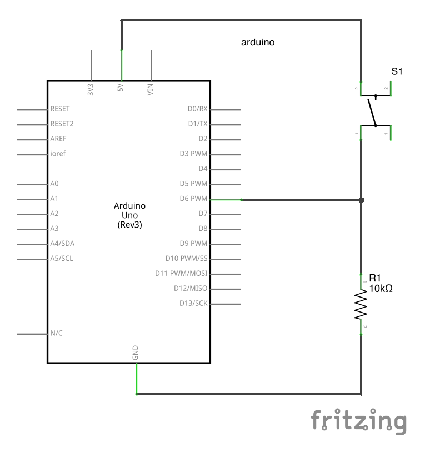
\includegraphics[width=0.7\columnwidth]{img/pulldown.eps}
 \end{minipage}
 \begin{minipage}{0.5\columnwidth}
  \centering
  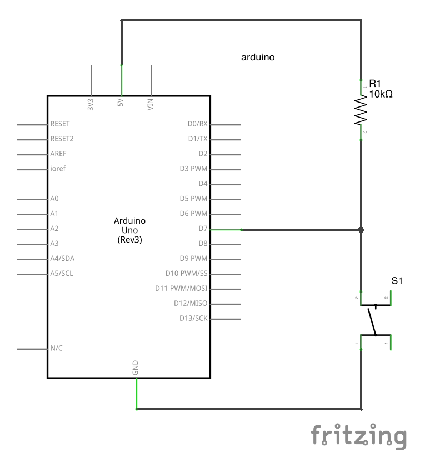
\includegraphics[width=0.7\columnwidth]{img/pullup.eps}
 \end{minipage}
  \caption{プルダウン抵抗 (左) とプルアップ抵抗 (右)}
\end{figure}


\section{PWMで明かりをコントロール}
\begin{lstlisting}
//LEDのフェードインとフェードアウト

import processing.serial.*;
import cc.arduino.*;
 
Arduino arduino;
int ledPin = 3;   //LEDが接続されたピン
int i = 0;        //カウントアップとダウンに使用
 
void setup() {
  size(400, 200);
  arduino = new Arduino(this, Arduino.list()[6], 57600);
  arduino.pinMode(ledPin, Arduino.OUTPUT);   //LEDのピンの出力に設定
}

void draw() {
  for (i = 0; i < 255; i++) {    //0から254までループ(フェードイン)
  arduino.analogWrite(ledPin,i); // LEDの明るさをセット
  delay(10);                     // 10ミリ秒停止 analogWrite()は一瞬なので
                                 // これがないと変化が目に見えない  
  }
  for (i = 255; i > 0; i--) { //255から1まで(フェードアウト)
    arduino.analogWrite(ledPin,i );
    delay(10);
  }
}
\end{lstlisting}

\section{光センサとは}
CdSセル: CdS(硫酸カドミウム)を主成分とする電子部品。
表面に当たる光の量に従って抵抗値が変化する。
周りが暗いと抵抗値が大きく、明るいと抵抗値が小さくなる。

\begin{itemize}
 \item \textbf{利点}
       \begin{itemize}
	\item 可視光線に対して高感度
	\item 小型で軽量
	\item 比較的安価
       \end{itemize}
 \item \textbf{欠点}
       \begin{itemize}
	\item 反応速度がやや遅め
	\item カドミウム = 有害物質
       \end{itemize}
\end{itemize}


\section{光センサを利用する}

\subsection*{TRY1: 回路を組み立ててみよう}
回路図を参考にして、光センサと Arduino を接続してみる。
その際必ず、Arduino は PC から取り外した状態で配線すること!

回路図

\subsection*{Analog Input}
Analog input の説明とコードをほげほげ


\subsection*{TRY2: Processing から Arduino の光センサ値を取得してみよう}
Processing から光センサの値を取得し光センサの値を観察しよう。

TRY1 で組み立てた回路を用いて、光センサの値を println を使って、ログに表示してみる。

[Hint 1]
println (表示したい値);

[Hint 2]

\begin{lstlisting}
 import processing.gainer.*;
 Gainer gainer;

 void setup(){
   gainer = new Gainer (this);
   gainer.???;
 }

 void draw(){
   ???(???);
 }
\end{lstlisting}


\subsection*{TRY3: センサの値をProcessingの画面にを表示してみよう}
先ほどはコンソール(Processing IDE の下の黒いところ)にセンサから取得した値を表示しましたが、次は Processing の画面に表示してみましょう。

\subsubsection*{Processing で画面に文字を表示する}
Processing で文字を表示するためには text() を用います。
\begin{lstlisting}
 void setup() {
   size(400, 300);
 }

 void draw() {
   // x = 50, y = 100 のところから "Interactive Art" の文字列を描く
   text("Interactive Art", 50, 100);
 }
\end{lstlisting}

また、 PFont を用いることによってフォントの種類を変更することができます。
\begin{lstlisting}
 PFont font;

 void setup() {
   size(400, 300);
 
   font = createFont("font_name", 32); // フォントの用意
   textFont(font, 24);
 }

 void draw() {
   text("Interactive Art", 50, 100);
 }
\end{lstlisting}

これらを利用して光センサから取得した値を画面に表示してみましょう。

% PFont myFont;
% PFont オブジェクトの宣言。
% プログラムの頭に書く。
% 複数宣言することで、違う種類のフォントを使用することができる。

%  myFont : PFont オブジェクトの名前
% createFont(“useFont”, 32);
%  フォントを作成し、PFontオブジェクトに読み込む命令。void setup の中に書く。
%   “useFont” : 使用したいフォント名 (Arial, MS Gothic, etc...)
%                   ※IDE上のタブのTools → Create Font... から 確認可能
  
% 数字
% : 作成するフォントのサイズ (大きくしすぎると、処理が重くなる。)
% textFont(myFont, 24);
%  使用するフォントの選択をする命令。
%   myFont = 使用するPFontオブジェクトの名前
%   数字 = フォントサイズの指定
% textAlign(LEFT);
%  文字の揃え位置を指定する命令。
%   LEFT
% : 左揃え(初期設定、宣言しなかった場合も)
%   CENTER : 中央揃え
%   RIGHT
% : 右揃え
% text(“hoge”, x, y);
 
%  文字を書く命令。
%   “hoge” : 表示文字列
%   x!! : x座標の位置
%   y!! : y座標の位置

\subsection*{TRY4}
TRY2、TRY3を参考にし、Processing の文字列 (text) で光センサの値を表示する。

[Hint]
\begin{lstlisting}
import processing.gainer.*;
Gainer myGainer;
PFont myFont;
void setup(){
	
size(???, ???);
	
colorMode(RGB, ???);
	
myGainer = new Gainer(this);
	
myFont = ??? (“Arial”, 24);
	
textFont(myFont);
	
textAlign( ??? );
	
myGainer.
???
;
}
void draw(){
	
background(?);
	
fill(???);
	
text(“value = ”+ myGainer.analogInput[0], ???, ???);
}
 
\end{lstlisting}

\end{document}